%
% This is an example file and is hereby explicitly put in the
% public domain.
%
\documentclass[ecp,tc,english]{iiufrgs}


% Use unicode
% pacote para acentuação
\usepackage[utf8]{inputenc}  
\usepackage[greek,english]{babel}

% Necessário para incluir figuras
\usepackage{graphicx}
% pacote para usar fonte Adobe Times
\usepackage{times}              
% pacote para usar citações abnt
\usepackage[alf,abnt-emphasize=bf]{abntex2cite}	

% Folha de capa
\title{Memory-resistor based computing}
\author{Hertzog}{Alexandre}
\author{Bringmann}{Oliver}
\author{Schweizer}{Thomas}
\author{Kühn}{Johannes Maximilian}
\author{Dobler}{Markus}
\author{Gerum}{Christoph}
\author{Braun}{Axel}
\advisor{Lima Kastenschidt}{Fernanda}

\date{December}{2015}
\location{Tuebingen}{Germany}
% Fim da folha de capa

%
% palavras-chave
% iniciar todas com letras minúsculas, exceto no caso de abreviaturas
%
\keyword{computing architecture}
\keyword{memristor}
\keyword{memory-resistor}
\keyword{non-Von Neumann architecture}

%
% inicio do documento
%
\begin{document}

% folha de rosto
% às vezes é necessário redefinir algum comando logo antes de produzir
% a folha de rosto:
% \renewcommand{\coordname}{Coordenadora do Curso}
\maketitle

% dedicatoria
\clearpage
\begin{flushright}
\mbox{}\vfill
{\sffamily\itshape
``If I have seen farther than others,\\
it is because I stood on the shoulders of giants.''\\}
--- \textsc{Sir~Isaac Newton}
\end{flushright}

% agradecimentos
\chapter{Agradecimentos}
Thanks to the Tübingen Universität colleages: Oliver Bringamann, Thomas Schweizer, Johannes Maximilian Kühn, Markus Dobler, Christoph Gerum and Axel Braun for all the help and wonderful insights about this project.

Thanks to the UFRGS people: Davi A. F., Juliano M. F., Karina V. M., Mateus F. D., Maurício K. B., Luigi V. F. and Paulo A. H. for the great friendship and showing me that it is okay to graduate late after all. These were some pretty long 7 years.

Thanks to the CTBM team: Gabriel A. L., Gabrihel S. V. João H. R. M. and Lucas S. K. for being present despite my distance.

To the WG43 family: Andreas H., Ian K., Lukas P. and Nara M. for being such awesome people, great drinkers, better-than-average cooks and warm germans in the cold weather.

Thanks to my family: Anelise H., Augusto H., Eleonor H., João B. H., Marlon M. G. and Mayra L. M. for the infinite strenght and willpower given to me.

And finally, thanks to my dearly loved girlfriend: Mayã O. M. for showing me that I can be a better person by knowing myself.

% resumo na língua do documento
\begin{abstract}

This document is about the theoretical use of memory-resistor elements to perform math operations, posing itself as a basic non-Von Neumann Architecture for a simple processor that is able to dispatch instructions to these elements. This thesis also presents some ideas for the optimization of these operations by making use of simple schedule optimizations.

\end{abstract}

% resumo na outra língua
% como parametros devem ser passados o titulo e as palavras-chave
% na outra língua, separadas por vírgulas
\begin{englishabstract}

Esse documento diz respeito ao uso teórico de elementos resistores de memória para executar operações matemáticas, se identificando como uma arquitetura não-Von Neumann básica para um processador que envia instruções para esses elementos. Essa tese também apresenta algumas ideias para a otimização dessas operações usando técnicas simples de escalonamento.

\end{englishabstract}

% lista de abreviaturas e siglas
% o parametro deve ser a abreviatura mais longa
\begin{listofabbrv}{DRAM}
	\item[DRAM] Dynamic Random Access Memory
	\item[HD] Hard Disk
	\item[SSD] Solid State Disk
\end{listofabbrv}

% lista de figuras
\listoffigures

% lista de tabelas
\listoftables

% sumario
\tableofcontents

% aqui comeca o texto propriamente dito

% introducao
\chapter{Introduction}
For a long time now we have been dealing with Von Neumann architectures in the last computer generations. Since the beginning, we count with a processor that gets from, processes and stores to a static and slower storage, being that a DRAM memory, an HD drive, a SSD drive or even a flash drive.

We use this architecture scheme because it is very expensive to create processing elements. It is logical to concentrate these processing elements in one or more cores and compensate the lack of storage speed by putting one or more levels of low capacity, high speed and expensive levels of cache. The slower a storare is, the cheaper it gets.

But since the 70's, it was predicted that there is another base electric component, called the memory-resistor, or memristor. This resistor is capable of "saving" input current up to a certain point, when it changes its resistivity from a high resistance value to a low resistance value in a non-volatile manner. If the variables involving this oscillatory behavior are known, it is possible to use memristors and be sure that their stored data is correct. The input current does not need to have predetermined intensities, nor needs a clock or oscillation mechanism, since a memory-resistor is an analog entity.

However, no one was able to reliably produce these elements up to recently. HP disclosed that it was actually possible in \cite{missingmr08}. There are researches of them being used as neural interfaces \cite{mrcrossbar11}, performing basic logic operations \cite{mrstatefullogic10} and even parallel researches regarding their use as a processing unit, although with a slightly different approach \cite{metastateswitches14}.

\chapter{Von Neumann Architectures}

For a long time now Von Neumann architecture has been ruling electronic devices, from smartphones to personal computers to supercomputers. This architecture defines that there is a central processing unit that will access a memory to fetch instructions of a given program and to store the results of its processing results. To deal with the rising of processing performance and power requirements of processors, they were split into many less powerful cores and the memory into more memory layers, with a very fast cache close to the processor, to the main DRAM and then to the HD that have relatively longer access times. There are more layers, but the idea of the architecture remains, as there is a processing center and a storage medium.

A new technology can break this paradigm by being the processing and storage medium at the same time. Memory resistors, also known as memristors, store current passing through them and, when there is a given amount of charge in them, they will change from a very high resistance state to a low resistance state. This predictable behavior makes them able to, under controlled circumstances, reliably perform mathematical operations. Since they also store this charge indefinitely and without exterior influence, they also serve as a great storage medium that is fast unlike HDs and does not need to be recharged like current DRAMs and, therefore, consumes less energy.

By developing a very simple processor that is able to dispatch inputs to these memristors logically, it is possible to use them in just the same way current generation processors are used. This dispatcher is very simple, since it doesn't need to actually do the computations, only send the instructions to the addressed memristors and they'll naturally perform these operations. This decentralized processing is a very good example of non Von Neumann architecture.

\chapter{Memory Resistors}

Memristor is a fundamental electrical component whose existence was predicted in 1971,by Leon Chua. Its main characteristic, memristance, links magnetic flux and charge, meaning that variations in charge change its magnetic flux, which in turn means that by changing the charge, it is possible to change its voltage drop-off. Because of that, it is feasible to consider that memristance is a resistance that depends on current, functioning basically as an integrator of charge. There are many papers that discuss their electrical details and such are beyond the scope of this document. In short, with some charge, a memristor will be on its high-resistance state, typically around hundreds of KΩ or MΩ, and after this charge surpasses a given amount, the memristor will change to its low- resistance state, which is around tens of KΩ.

The decision level is the resistance in which there is a distinction between high- resistance and low-resistance.

Before any further details about its logical function, there are a couple concepts that must be understood: pulse and base. Pulse is the name given to the square voltage pulse applied to a memristor input port. A pulse does not need to have strict height or length, as such properties can be defined on-the-fly as is more convenient to the application. Base is the amount of pulses of same height and length a memristor needs to change its state. For example, if it is defined that a memristor needs ten pulses of length “l” and height “h”, its base is ten. By being analog components, the only practical limit to this base property is defined by the memristor construction methods and input circuitry precision, meaning that a memristor can have a base as low as 1 and as high as thousands.

\chapter{Memristor as a processing component}

Basic operations for memories are read and write. It is not different when it comes to memristors, although it differs a lot from the same operations in current random access memory architectures.

To write to a memristor, the base must be informed. With that base, the input voltage is defined in function of the desired value, following the formula:

\begin{equation}
  voltage = \frac{value}{base} + basevoltage
\end{equation}

Due to electrical characteristics of the memristor, voltages below 3V are absorbed by the memristors energy dissipation while in high-resistance mode. Therefore, it is necessary to introduce a “basevoltage” constant that makes sure that the desired value is correctly represented when it is inputted to the memristor.

\begin{figure}
  \caption{Base versus voltage of input pulses.}
  \centerline{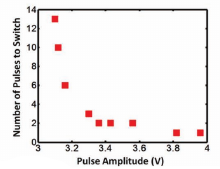
\includegraphics{fig/memristor-basexvoltage.png}}
  \legend{Source: [TODO]}
  \label{fig:mr_bxv}
\end{figure}

After base times value $ base * value $ pulses to a memristor, it will chatge and change to the low-resistance state. It is necessary to reset the memristor when it is on this state, since anything inputted to it in this state will be lost. To avoid the need to reset the memristor everytime it switches, there is a feedback from its output voltage to its input. The voltage spike generated, when fed back, is enough to reset it back to the high-resistance state, where input values are stored.

\begin{figure}
  \caption{Graph showing the resistance versus the amount of pulses at base 10.}
  \centerline{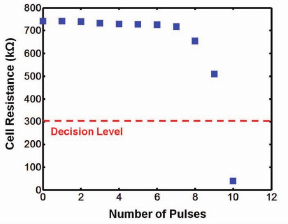
\includegraphics{fig/memristor-resistancexpulses.png}}
  \legend{Source: [TODO]}
  \label{fig:mr_rxp}
\end{figure}

The write process may consist of two types: full value loads and partial value loads. Full value loads are used to write a value in a memristor in a single cycle, by using higher pulse heigths than that base specified. This is useful to cut down load times, but if the value is bigger than the base, the excess value will be lost, with only one overflow count. Partial value loads usually are unitary pulses, which increment in one the memristor value in the current base. With this method no value is ever lost, since the memristor resets fast enough to have its overflow counted and to store the next input. This makes the write operations extremally slow for large values.

\begin{figure}
  \caption{Inputting three unitary pulses into a memristor that contains no value.}
  \centerline{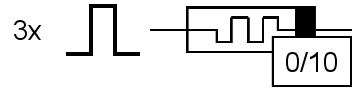
\includegraphics{fig/memristor-basicwrite.png}}
  \legend{Source: Author}
  \label{fig:mr_basicwrite}
\end{figure}

\begin{figure}
  \caption{Result of the write.}
  \centerline{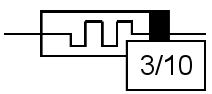
\includegraphics{fig/memristor-basicwriteresult.png}}
  \legend{Source: Author}
  \label{fig:mr_basicwriteres}
\end{figure}

To read a memristor value, it is necessary to apply and count pulses to it until it goes into low-resistance state. The count value is the inverse of the value previously stored, considering the base. The problem with reading a value is that it actually destroys the value, since it is not possible to deduce the value only by reading its current resistance as the only voltage distinction is the difference between low-resistance and high-resistance. The read value is saved in a buffer. If that value is needed for another operation, it is necessary to re-input it after the read process.

\begin{figure}
  \caption{Reading from the previous example. $ N=7 $ in this case.}
  \centerline{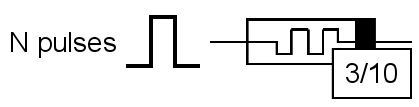
\includegraphics{fig/memristor-basicread.png}}
  \legend{Source: Author}
  \label{fig:mr_basicread}
\end{figure}

It is worth noting that the bigger a memristor base is, the longer it may take to read its value. For example, if a memristor has a stored value of 3 in base 10, it takes 7 cycles to read this value, since it is necessary to apply 7 pulses until it changes state. However, if another memristor has a stored value of 3 in base 100, it takes 97 cycles to read the same value.

The process of a memristor changing from high-state to low-state is called overflow, since it represents the amount of times that value has exceeded the memristor storage capacity.

\chapter{Performing mathematical operations}

Now that the read and write mechanisms are explained, it is possible to elaborate algorithms that perform basic mathematical operations. Four operations will be described: plus, minus, multiplication and division. The first three ones were described by David Wright.

[TODO] ref

\section{ADD operation}

The plus operation is the most straight-forward of them. To do it, it is necessary to just write the first operand to a memristor and then write the second operand in to the same memristor. This memristor will contain the result of the operation. To get this value, the memristor is read and this value is inverted.

\begin{figure}
  \caption{Example of a sum using memristors.}
  \centerline{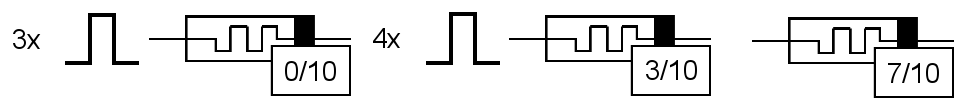
\includegraphics{fig/basicadd.png}}
  \legend{Source: Author}
  \label{fig:basicadd}
\end{figure}

\section{SUB operation}

To perform the minus operation, two memristors are necessary. In the first step, the first operand is written in the first memristor and the second operand is written on the second memristor. The first memristor is read and this value is written in the second memristor. The subtraction result is the value read from the second memristor.

\begin{figure}
  \caption{Sample operation of 7-3. M is the amount of pulses to memristor A reset and N=4 is the result.}
  \centerline{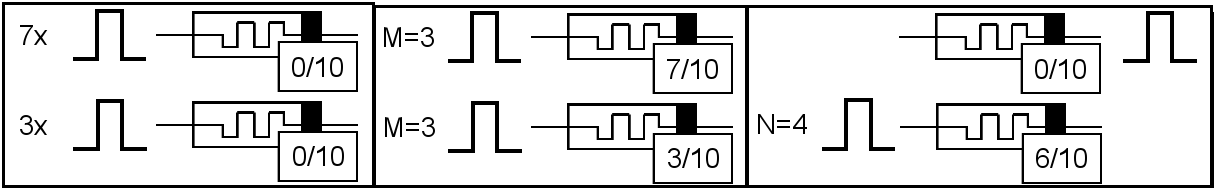
\includegraphics{fig/basicsub.png}}
  \legend{Source: Author}
  \label{fig:basicsub}
\end{figure}

\section{DIV operation}

Division operations can be very efficient in memristors, because they use the memristors core principle to their advantage. To do it, the base is defined as the divisor and then the dividend is written. The amount of times the memristor changed to low state indicates the quotient and the rest is represented by the inverted value saved in this memristor.

\begin{figure}
  \caption{Dividing 10 by 3. The “3x” on the right is the amount of overflows and the 1 inside the memristor is the remainder.}
  \centerline{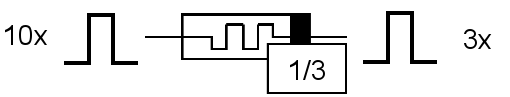
\includegraphics{fig/basicdiv.png}}
  \legend{Source: Author}
  \label{fig:basicdiv}
\end{figure}

\section{MUL operation}

These operations are based on a very common principle in the binary computing that to multiply by two, a simple bit-shift operation is applied. That same principle is valid to memristors, the difference is that they are not limited to base two.

To perform that, the first operand is written in a memristor with base equal to the second operand and the amount of times the memristor overflowed are written in a second memristor of base equal to second operand as well. If this second memristor overflowed as well, these values are written to a third memristor in the same fashion as they were on the second memristor case. Upon reading, these values are read interpreting them a digit higher than they were inputted.

For example, $ 5 * 3 $:

\begin{itemize}
    \item Write 5 into a memristor[0] with base 3;
    \item The result is a stored value of 2 plus 1 overflows;
    \item One overflow is written in the memristor[1] of base 3;
    \item Shifting the digit, the first memristor that could be intepreted as $ 3^0 $, is now $ 3^1 $ and the second is $ 3^2 $;
    \item The final result is $ 2*3^1 + 1*3^2 = 6+9 = 15 $.
\end{itemize}

If a multiplier is small and the use of multiple memristors to store this result is impractical, another technique could be used. The multiplier could define the base of an auxiliary loop-control count memristor. This memristor would be incremented and the multiplicand value would be written in the destination memristor. When the loop-control memristor overflows, the multiplicand is inputted one last time and the operation finishes. This is basically the multiply two values by the multiple additions method.

\begin{figure}
  \caption{5x3 multiplication with counting memristor. Before this operation completes, the second memristor would overflow once and end with a value of 5.}
  \centerline{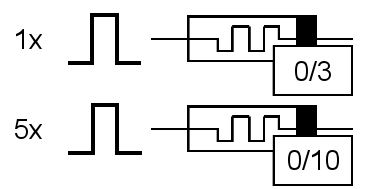
\includegraphics{fig/basicmul.png}}
  \legend{Source: Author}
  \label{fig:basicmul}
\end{figure}

\chapter{Architecture and implementation}

All the described hardware, implementations and algorithms below were implemented using the SystemC plug-in for C++. All modules are asynchronous, which means that they don't require an external clock to function. This was deliberate to better emulate the behavior of memristor and memristor-dependent hardware, since the former is analog and asynchronous.

It is also worth noting that all inputs and outputs are implemented as digital signals. That applies even to real world analog values, the memristor input voltage and memristor output resistance. It is supposed to emulate these properties, and not to actually be one of them. That would require the use of more complex libraries to the implementation of analog devices and such task adds a lot of complexity to this work.

Also, all components, except for the memristor and their input and output managers at the Memristor Memory Array are supposed to be digital. One of the main points of this document is to present a viable architecture that is a hybrid model between digital circuitry and analog memristors.

\begin{figure}
  \caption{Overall architecture.}
  \centerline{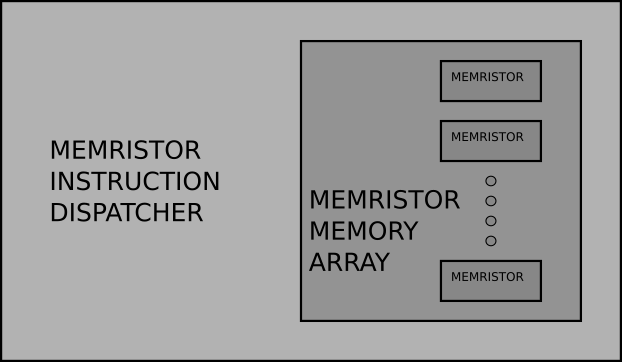
\includegraphics{fig/arch.png}}
  \legend{Source: Author}
  \label{fig:arch}
\end{figure}

\section{Memristor instruction dispatcher (MID)}

This is the hardware that launches the instructions to the Memristor Memory Array. It is capable of handling plus, minus, division and multiplication operations, as described in the previous section. Logical operations, such as AND, NAND, OR, NOR and comparison operations can be easily implemented, but, for the sake of complexity in this document were left out.

Its inputs are:

\begin{itemize}
    \item Operand 1 and Operand 2: operands of an operation;
    \item Base: base to perform the operation; it is ignored when performing multiplication and division;
    \item Operator: the operation to be performed;
    \item Reset: resets the state of the dispatcher and memory;
    \item Perform Operation: start performing an operation.
\end{itemize}

Its outputs are:

\begin{itemize}
    \item Result: result of the operation;
    \item Overflow: count of overflows that happened during that operation;
    \item Operation done: indicates that the current operation finished.
\end{itemize}

The MID will execute the operations whenever the “Perform Operation” input changes, performing similarly to a latch-based system. When that event happens, it will first read the reset pin and, if it is the case, it will replicate the reset signal to its components and reset itself. Otherwise, it will read the other inputs and perform the requested operation.

When this operation finishes, the “Operation done” pin is changed after the result and overflow values are assigned to their respective output pins.These values are read directly from the outputs of the Memory Array.

\begin{figure}
  \caption{MID I/O pins.}
  \centerline{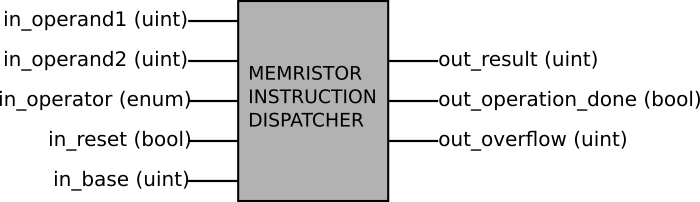
\includegraphics{fig/mid.png}}
  \legend{Source: Author}
  \label{fig:mid}
\end{figure}

\section{Memristor memory array (MMA)}

Is contained inside the MID unit. The MMA has many creation-defined addressable memristors. It manages the memristors input voltages, monitors their outputs and counts the amount of overflows that happened to the active memristors (the ones that are being used during an operation). Addresses, write data, read data and base are serial parameters, which are read in a bundle every time any of them changes.

Its inputs are:

\begin{itemize}
    \item Perform operation: request to perform an operation;
    \item Read/Write: indicates whether the operation is a read or a write;
    \item Quantity: amount of addresses and write data to be received;
    \item Addresses: addresses to be read or written;
    \item Write data: data to be written; is not used the current operation is read;
    \item Base: base of the operation;
    \item Reset: resets the state.
\end{itemize}

Its outputs are:

\begin{itemize}
    \item Operation done: indicates that the operation finished;
    \item Read data: serially emitted values read from a subset of memristors;
    \item Overflow: amount of overflows that happened during write operation.
\end{itemize}

Upon receiving an operation request via “Perform operation”, it will read “Addresses”, “Write data” and “Base” an amount of times equal to “Quantity”, unless “Reset” is true, in which case it resets its components and itself. After reading the inputs, it will define what is the current operation.

If the operation is a write, MMA will generate and send the pulses to all indicated memristor addresses with the values in the write data buffer, respectively and in parallel. While it is inputting to the memristors, it is counting the amount of overflows happening in the active ones. Once the write is finished, it will gather the amount of overflows and output them along with an “Operation done” signal.

It the operation is a read, it will apply pulses to all the memristor in the address array. If one of them changes state, it will stop sending pulses to that memristor. This continues until all of them have reset only once, then it gathers the data in its buffers and queues them in the output buffer and sends them.

All the buffers in the MMA are meant to be pure-digital buffers. In the case of the input buffer, when a value is read, it's pulse value interpreted and then sent to the respective memristor.

\begin{figure}
  \caption{MMA I/O pins.}
  \centerline{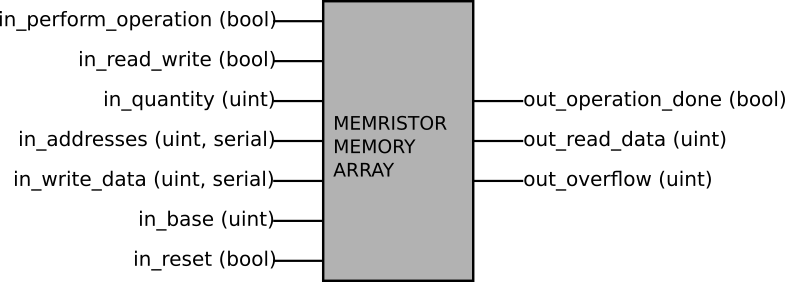
\includegraphics{fig/mma.png}}
  \legend{Source: Author}
  \label{fig:mma}
\end{figure}

\section{Memristor}

Gets instantiated in the MMA module. It is a very simple accumulator module, which reads the value on the input, adds it to an existing variable that represents the accumulated energy and, depending on its value, outputs either a high value that represents a high resistance or a low value that represents a low resistance.

If this accumulated value surpasses the maximum threshold, the module automatically resets this value, to emulate the feedback behavior. This is done just in time that the low-resistance pulse gets sent to the output and is detectable by the MMA.

\begin{figure}
  \caption{Memristor I/O pins.}
  \centerline{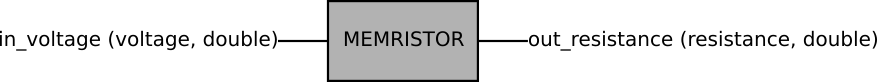
\includegraphics{fig/mrarch.png}}
  \legend{Source: Author}
  \label{fig:mrarch}
\end{figure}


\chapter{Multi-base operations}

As seen previously, some operations, specially plus and minus can have a pretty big latency, due to base reasons. If an instruction requires that a plus operation is performed in base 100, in some cases it may take a long time to read the value contained in that memristor, depending on the values previously stored.

With that in mind, it was developed a method in which memristors will represent “digits” of a number in a given base, instead of storing the absolute value. The same base-100 operation could be split into three memristors of base-10, for example, and have its latency greatly reduced.

It is worth noting that none of this is done by the MID or the MMA. This is all done in software which is, in this case, a given set of instructions passed to the MID. When generating this executable code, it is up to the compiler to split the otherwise large base operations into multiple smaller base operations that are computed at the MMA. There is no compiler implemented so far. All the programs used to test the MID were hard-coded into the upper level of the simulation.

\section{Multi-base plus}

Before the software inputs the instructions to the MID, it must be decomposed into as many operations of smaller bases as is needed, defined by the compiler. These operations are then forwarded to the MID which processes them normally, unaware that the current set of operations are actually a single operation.

To do so, both operands are split according to its digits, or in any other advantageous way. These operands are then forwarded to the MID, each with its respective digit counterpart. The overflow values are re-inputted as normal operands for the next digit which also receives the second part of the operands. This process is repeated for every digit, until none remain. The final result is read from all the memristors and a weight is given to each of these values, according to what was previously defined, along with the overflow values, which happen when there were not enough memristors to compute the operation.

Since the normal plus process only takes one memristor for every two operands and the multi-base plus does not need additional memristors, the amount used in this process is equal to the amount of digits split by the compiler. There could be a very reasonable speed up, varying from case to case.

An example of multi-base sum is the operation below. Note that the number inside parenthesis are number computed in individual memristors.

$ 153b10 + 78b10 = (1+0)*10^2 + (5+7)*10 + (3+8) $

$ = 1*10^2 + (2 + 1 overflow)*10 + (1 + 1 overflow) $

$ = 1*10^2 + (2 + 10)*10 + (1 + 10) = 231 $

\section{Multi-base minus}

Very similar to the multi-base plus. The difference is that the overflows are decremented from the next digit, instead of adding to it.

When a minus operation is computed and an overflow happened, it means that the second operand was greater than the first operand. Therefore, when the current digit is smaller than its couterpart, the overflow must carried to the next digit and subtracted from that result. After all digits were processed, the result and the amount of overflows (that happen when the second operand was bigger than the first one) are outputted considering the weight of each memristor.

Like the multi-base plus, the minus operation does not need additional memristors to perform operations. Since every digit takes two memristor the subtraction, to perform this operation it is necessary to have double the amount of digits in memristors.

Below there is an example of multi-base subtraction.

$ 137b10 - 65b10 = (1-0)*10^2 + (3-6)*10 + (7-5) $

$ = 1*10^2 + (7 + 1 overflow)*10 + 2 $

$ = 1*10^2 + (7 - 10)*10 + 2 = 72 $

\chapter{Results}

From the simulations, it was possible to get some information regarding cycles per operation, which is documented in the tables below. These cycles are the latencies of multi-base plus and minus.

All the comparisons are done cycle-wise and, again, it is very important to point out that memristors don't need to have a frequency of operation as low as nowadays computers have. Since they are analog entities, it is just a matter of how much precision the digital circuitry that interfaces with them has.

[TODO] tabela 1
Table 1. Results from the multi-base plus.

In the “Split” column, numbers inside parenthesis are how that operand was split for the number in “Base”. Read-write cycles are represented in a read or write code followed by the amount of cycles that operation took and operations per memristor are separated by semi-colons. Finally, the “Total” column has the total amount of cycles per memristor. Considering that these operations can be performed in parallel in all memristors with post process carry-computation, the latency of that operation would be the greater number in the “Total” column.

[TODO] tabela 2
Table 2. Cycle results fro the multi-base minus.

\chapter{Conclusion}

Memristor use is a very promising up-and-coming technology. Their storage functionality could fill the very large gap that exists between processors and storage mediums. Even though this technology is just beginning, its potential is very good and the architecture presented here still has a lot room for growth.

They can bring great benefits in some areas in which transistor technology has little advantages. Neural networks is a field that could expand really fast, along with brain simulations. Even when it comes to short term benefits, current permanent storage devices could also make a great use of them, with some studies from HP that clock memristor to a tenth of DRAM speeds.

[TODO] tabela 3
Table 3. Overall comparison between memristors and DRAM memory.

\bibliographystyle{abntex2-alf}
\bibliography{biblio}

\end{document}
